% WACV 2027 review manuscript
\documentclass[10pt,twocolumn,letterpaper]{article}
\usepackage[algorithms]{wacv} %review,
%
% --- inline annotations
%
\newcommand{\red}[1]{{\color{red}#1}}
\newcommand{\todo}[1]{{\color{red}#1}}
\newcommand{\TODO}[1]{\textbf{\color{red}[TODO: #1]}}
% --- disable by uncommenting
% \renewcommand{\TODO}[1]{}
% \renewcommand{\todo}[1]{#1}

\usepackage{caption}

\usepackage{graphicx}
\usepackage{booktabs}
\usepackage{multirow}
\usepackage{amsmath,amsfonts,amssymb}
\usepackage{microtype}
\usepackage{xcolor}
\usepackage{enumitem}
\usepackage{siunitx}
\usepackage{array}
\usepackage[utf8]{inputenc}
\usepackage[T1]{fontenc}
\definecolor{wacvblue}{rgb}{0.21,0.49,0.74}
\usepackage[pagebackref,breaklinks,colorlinks,allcolors=wacvblue]{hyperref}

\newcommand{\method}{\textsc{EvoMem3D}}
\newcommand{\R}{\mathbb{R}}
\newcommand{\rednote}[1]{\textcolor{red}{\textbf{[Missing: #1]}}}
\def\wacvPaperID{780}
\def\confName{WACV}
\def\confYear{2027}



\newcommand\mk[1]{\textcolor{cyan}{(\textbf{Moshe}: #1)}} 
\newcommand\yi[1]{\textcolor{cyan}{(\textbf{Yotam}: #1)}} 


\title{EvoMem3D: Adaptive-Depth Temporal Representation Memory for Multi-Camera 3D Detection}

% \title{EvoMem3D: Trading Transformer Depth Across Time
% for Multi-Camera 3D Detection}

\author{Moshe Kimhi$^{1,2}$
\and Idan Kligvasser$^{1}$
\and Yotam Intrator$^{1}$
\and Regev Cohen$^{1}$
\and Ehud Rivlin$^{1,2}$
\\
$^{1}$Google Research \quad $^{2}$Technion}

\begin{document}
\maketitle


\begin{abstract}
Deep vision-transformer backbones dominate the inference cost of
multi-camera 3D detectors, although adjacent driving frames often
require only limited changes to the detector's high-level scene
representation. We introduce \method{}, which treats the
detector-interface representation as recurrent temporal state and
allocates transformer depth to each incoming frame. A full-depth
action refreshes the state, whereas a partial action projects an
intermediate transformer representation to the detector interface
and applies a lightweight gated correction to the existing memory.
A controller uses online ego-motion, previous detection summaries,
memory state, and an early-feature change cue to choose among
encoder blocks 8, 12, 16, and 24. Geometry-dependent detector
encoding is recomputed from the current camera calibration and ego
pose at every timestamp rather than being propagated through memory.

On nuScenes, a DETR3D--EVA-02-L baseline obtains 61.90 NDS and
53.10 mAP at 373.4 ms per frame. \method{} obtains 60.43 NDS and
54.41 mAP at 189.6 ms, a $1.97\times$ speedup. These results indicate that temporal representation memory and adaptive encoder depth are complementary mechanisms for reducing
repeated computation in streaming 3D detection.
\end{abstract}


% \begin{abstract} Large vision-transformer backbones account for a substantial fraction of the inference cost of multi-camera 3D detectors, although adjacent driving frames often require only limited changes to the detector's high-level image representation. We introduce \method{}, which treats the dense detector-interface feature as recurrent temporal memory and allocates transformer depth independently at each timestamp. A full-depth action refreshes this memory, whereas a partial action projects an intermediate transformer representation through a learned depth-specific feature pyramid and applies a lightweight gated correction to the existing state. Before encoding frame $t$, a compact policy chooses among blocks 8, 12, 16, and 24 using relative ego-motion, scene and memory age, previous detection summaries, and lagged shallow-feature drift measured between frames $t-2$ and $t-1$. The memory is stored before detector-side positional and geometric conditioning; the detector therefore receives the current intrinsics, extrinsics, ego pose, and image metadata at every timestamp. The memory nevertheless remains defined on the camera image grids, and current partial features and periodic full refreshes are used to correct accumulated spatial and semantic error. On nuScenes, full DETR3D--EVA-02-L inference obtains 61.90 NDS and 53.10 mAP at 373.4 ms per frame. The accuracy-oriented \method{} configuration obtains 60.43 NDS and 54.41 mAP at 195.7 ms, a $1.91\times$ speedup. A faster operating point obtains 60.43 NDS and 51.37 mAP at 189.6 ms, a $1.97\times$ speedup. Fixed-depth and updater ablations show that shallow current features are substantially more effective when used to correct persistent high-level memory than when used alone. Representation analysis further shows that final-feature drift is predictable from signals available before current-frame encoding, enabling computation to be allocated according to temporal scene change. \end{abstract}


\section{Introduction}

Modern camera-only 3D detectors increasingly rely on large
vision-transformer backbones to extract strong multi-view image
features. Although temporal detector heads can propagate BEV features
or object queries across frames, the image backbone is typically
executed at full depth for every timestamp. This uniform computation
ignores a defining property of driving video: the high-level scene
representation often changes more slowly than the raw images.

The central question is not whether an intermediate transformer
feature can replace a final feature. In general, it cannot: shallow
representations contain current visual evidence but lack the semantic
depth expected by the detector. Instead, we ask whether shallow
current-frame evidence can \emph{correct} a high-level representation
carried from previous frames. This view turns the detector-interface
representation into recurrent state. Full encoding periodically
refreshes that state, while partial encoding supplies an innovation
that updates only the parts of the state affected by the current
frame.

We introduce \method{}, an adaptive-depth temporal representation
memory for multi-camera 3D detection. At timestamp $t$, a lightweight
policy selects an encoder exit before the current images are
processed. A full-depth action replaces the memory with the current
final representation. A partial action projects an intermediate
representation to the detector interface and uses it as an innovation
that corrects the existing memory. Consequently, the state at time
$t$ combines the last full-depth representation with partial evidence
accumulated over the subsequent frames.

The policy is based on the observation that the amount of useful
current-frame computation is related to representation drift. Under
a common full-refresh interval, shallower exits degrade more strongly
when the final encoder representation changes substantially, whereas
stable intervals tolerate shallower updates. We therefore train a
small MLP to predict ordered drift classes using information available
before encoding frame $t$: relative ego motion, normalized scene age,
memory age, previous detections, and the L8 representation change
observed between frames $t-2$ and $t-1$. The corresponding class
selects one of the L8, L12, L16, or L24 actions.

Our experiments address three questions. First, does temporal memory
improve over current partial features alone under the same depth and
refresh schedule? Second, does representation drift identify frames
on which shallow encoding is insufficient? Third, can this drift be
predicted from deployable temporal signals? On nuScenes, \method{}
nearly halves end-to-end latency while retaining 97.6\% of the
full-depth NDS; its accuracy-oriented operating point additionally
exceeds the full-depth mAP in the evaluated run.

Use the following contributions:

Our contributions are:
\begin{itemize}[leftmargin=*]
    \item We formulate the dense pre-geometry image representation of
    a multi-camera 3D detector as recurrent temporal memory. Partial
    transformer representations are projected to the detector
    interface and used to correct this high-level state.

    \item We introduce a pre-encoding depth policy that predicts
    full-representation drift from relative ego motion, sequence and
    memory state, previous detections, and lagged L8 feature change,
    without evaluating additional current-frame transformer blocks.

    \item We empirically connect representation drift to the loss
    induced by insufficient encoder depth, and analyze which online,
    lagged-feature, and oracle signals predict this drift.

    \item On nuScenes, \method{} obtains 60.43 NDS and 54.41 mAP at
    a $1.91\times$ speedup, with a faster configuration reaching a
    $1.97\times$ speedup.
\end{itemize}





\begin{figure*}[t]
    \centering
    \includegraphics[width=\linewidth]{figures/paradigm.png}
    \caption{Overview of \method{}. Partial encoding supplies current-frame evidence, while cached dense features retain high-level context. The policy chooses encoder depth before the detector head is evaluated.}
    \label{fig:overview}
\end{figure*}




\section{Related Work}

\paragraph{Camera-only 3D detection.}
DETR3D samples multi-view features using projected 3D reference points, whereas PETR transforms 3D position information into the perspective-view feature domain \cite{wang2022detr3d,liu2022petr}. BEVFormer and BEVDet4D aggregate temporal evidence in bird's-eye view \cite{li2022bevformer,huang2022bevdet4d}. StreamPETR maintains object-query memory and processes long sequences online \cite{wang2023streampetr}. SparseBEV shows that sparse queries can provide a strong accuracy--efficiency balance \cite{liu2023sparsebev}. These approaches preserve temporal information at the BEV or object level. \method{} instead maintains the dense image representation before the 3D head, so it can reduce repeated backbone depth while leaving detector-side temporal modeling intact.

\paragraph{Efficient vision transformers.}
Recent efforts to accelerate ViT backbones in multi-view 3D detection largely focus on spatial token compression. Works such as ToC3D \cite{zhang2024toc3d} and SEPatch3D  \cite{SEPatch3D} leverage historical queries or temporal priors to segment and route salient foreground tokens. Similarly, SToRe3D \cite{store3d} introduces a planner-aligned framework that jointly sparsifies 2D image tokens and 3D queries based on future relevance. While these methods successfully reduce intra-frame spatial redundancy (the ``width'' of the network), they still require propagating the retained tokens through the entire network depth. Furthermore, although leading temporal frameworks like StreamPETR \cite{wang2023streampetr} efficiently propagate state via sparse object queries, they continue to execute a full-depth image backbone at every frame. In contrast, \method{} introduces \emph{temporal depth allocation}. By adaptively exiting the backbone early over time rather than strictly reducing spatial resolution, our approach addresses the dense backbone bottleneck orthogonally. Thus, maintaining a dense feature interface makes \method{} highly complementary to existing spatial token compression techniques.


\paragraph{Temporally distributed and adaptive-depth computation.}
TDNet distributes shallow subnetworks across consecutive video
frames and recomposes their features into a high-level representation
using temporal alignment \cite{hu2020tdnet}. Dynamic ViT methods such
as AdaViT and LGViT allocate transformer blocks or introduce
input-dependent early exits \cite{meng2021adavit,xu2023lgvit}.
\method{} lies at the intersection of these directions: it allocates
encoder depth over time while maintaining a recurrent representation
in the interface expected by a multi-camera 3D detector. Unlike a
standalone early-exit prediction, each partial representation acts as
an innovation that corrects persistent high-level state.


\paragraph{Feature reuse in video.}
Deep Feature Flow evaluates a costly network on keyframes and propagates deep features to nearby video frames \cite{zhu2017dff}. Our setting differs because synchronized cameras, current calibration, and a geometry-aware detector must remain consistent. Rather than relying on propagated stale features alone, \method{} evaluates a prefix of the current transformer and learns a correction in the detector's feature space.

\paragraph{Representation drift.}
Representation similarity provides a training signal for deciding when cached features are no longer sufficient. We use global cosine similarity and patch-token centered kernel alignment (CKA), which compares representation geometry and is less sensitive to some feature-space transformations \cite{kornblith2019cka}. These metrics supervise or diagnose the policy; end-to-end detection metrics determine whether the selected computation is useful.

\section{Method}
\label{sec:method}

\subsection{Temporal Representation Memory}

Let $I_t=\{I_t^v\}_{v=1}^{V}$ denote the synchronized camera images
at timestamp $t$. We decompose the detector into an image encoder
$E=E_{1:L}$, a feature-pyramid projector $N$, and a geometry-conditioned
detection head $D$. Full-depth inference is
\begin{align}
A_t &= N(E_{1:L}(I_t)),\\
\widehat{Y}_t &= D(A_t;\gamma_t),
\end{align}
where $\gamma_t$ contains the current image metadata, camera
intrinsics and extrinsics, ego pose, and the remaining detector-side
geometric inputs.

\method{} maintains a dense recurrent state $M_t$ in the same
multi-scale feature space as $A_t$. The state is stored before
detector-side positional and geometric conditioning. In our DETR3D
adapter, this interface is explicitly marked as
\texttt{memory\_is\_pre\_pe=True}; current $\gamma_t$ is supplied to
the head whenever $M_t$ is decoded.

For a partial action $a_t=\ell<L$, we compute
\begin{align}
H_t^\ell &= E_{1:\ell}(I_t),\\
C_t^\ell &= \Pi_\ell(H_t^\ell),\\
M_t &= U(M_{t-1},C_t^\ell),
\end{align}
where the learned depth-specific projector $\Pi_\ell$ maps the
intermediate tokens to the four-scale, 256-channel interface expected
by DETR3D. The same update module $U$ is shared across partial depths.
For a full-depth action,
\begin{equation}
M_t=A_t.
\end{equation}
The current prediction is always computed using
\begin{equation}
\widehat{Y}_t=D(M_t;\gamma_t).
\end{equation}

Let $\tau_t$ denote the most recent full-depth refresh. By recursion,
\begin{equation}
M_t =
\mathcal{M}\!\left(
A_{\tau_t},
C_{\tau_t+1}^{a_{\tau_t+1}},
\ldots,
C_t^{a_t}
\right).
\end{equation}
Thus, $M_t$ represents the interval from the most recent full refresh
through the current timestamp rather than the representation of one
particular frame. We define the memory age as
\begin{equation}
k_t=t-\tau_t
\end{equation}
and force a full refresh when $k_t$ reaches the configured maximum.

\paragraph{Current geometry and image-grid memory.}
Storing $M_t$ before detector-side geometric conditioning prevents
the system from caching a feature together with stale 3D positional
information. At frame $t$, the detector instead uses current
intrinsics, extrinsics, ego pose, and image metadata. This does not
make the memory invariant to image-plane motion: a feature at camera
$v$ and location $(h,w)$ at time $t-1$ is not guaranteed to describe
the same physical point at time $t$. \method{} addresses this
remaining discrepancy through current partial evidence, the learned
update gate, and a bounded memory age rather than claiming explicit
geometric transport.

\subsection{Depth-Conditioned Gated Memory Correction}

For feature-pyramid level $s$, we concatenate the previous memory and
the projected current representation:
\begin{align}
X_t^{\ell,s} &= [M_{t-1}^s;C_t^{\ell,s}],\\
G_t^{\ell,s} &=
\sigma\!\left(W_g^s * X_t^{\ell,s}\right),\\
R_t^{\ell,s} &=
W_r^s * X_t^{\ell,s},\\
M_t^s &= M_{t-1}^s+
\alpha_s G_t^{\ell,s}\odot R_t^{\ell,s}.
\end{align}
Here, $W_g^s$ and $W_r^s$ are $1\times1$ convolutions and
$\alpha_s$ is a learned residual scale initialized to zero. The
depth-specific projectors learn to express L8, L12, and L16 features
in a common detector-interface space, while the shared updater
determines where and how strongly that representation should correct
the previous memory. The gate can preserve stable content and
suppress stale memory when the current partial representation
disagrees with it, but it does not perform explicit spatial warping.

% The gate $G_t^{\ell,s}$ determines the spatial locations and channels
% that receive a correction, while the signed residual
% $R_t^{\ell,s}$ determines the content of that correction.
% The operation does not perform explicit geometric warping; instead,
% it learns to preserve stable memory and overwrite or suppress stale
% content using current-frame evidence.


\subsection{Pre-Encoding Depth Policy}

The policy is evaluated before encoding the current frame. Its input
is
\begin{equation}
q_t =
\left[
e_t,\;
r_t,\;
p_{t-1},\;
d_{t-1}^{8},\;
k_t,\;
\operatorname{onehot}(a_{t-1})
\right],
\end{equation}
where $e_t$ contains relative ego-motion variables, $r_t$ is the
normalized frame index since the beginning of the current scene,
$p_{t-1}$ summarizes previous detections, and $k_t$ is memory age.

The lagged shallow-feature drift is computed from cached L8
representations:
\begin{equation}
d_{t-1}^{8}
=
\frac{1}{V}\sum_{v=1}^{V}
\left[
1-
\cos\!\left(
\operatorname{pool}(H_{t-1}^{8,v}),
\operatorname{pool}(H_{t-2}^{8,v})
\right)
\right].
\end{equation}
Every candidate action executes at least eight blocks, so
$H_{t-1}^{8}$ is already available from the preceding inference
step. The signal therefore adds memory storage but no current-frame
encoder computation. It acts as a lagged estimate of how quickly the
visual representation is changing.

A two-layer MLP predicts
\begin{equation}
p_\theta(a_t\mid q_t)
=
\operatorname{softmax}
\left(
W_2\operatorname{ReLU}(W_1q_t)
\right),
\qquad
a_t\in\{8,12,16,24\}.
\end{equation}

\subsection{Representation-Drift Supervision}

Let $H_t^{L,v}$ be the final encoder representation for camera $v$.
We define full-representation drift as the mean camera-wise cosine
distance:
\begin{equation}
d_t^{L}
=
\frac{1}{V}\sum_{v=1}^{V}
\left[
1-
\frac{
\left\langle
\operatorname{vec}(H_t^{L,v}),
\operatorname{vec}(H_{t-1}^{L,v})
\right\rangle
}{
\|\operatorname{vec}(H_t^{L,v})\|_2
\|\operatorname{vec}(H_{t-1}^{L,v})\|_2
}
\right].
\end{equation}
The frozen full encoder is used only during policy-label generation.
Thresholds partition $d_t^L$ into four ordered classes corresponding
to L8, L12, L16, and L24, with larger drift assigned to deeper
encoding. The full-depth target path is not evaluated when the
deployed policy selects an action.

We use the mean across cameras because it provides the strongest
overall downstream policy behavior among the evaluated camera
aggregations. We separately analyze minimum-camera similarity,
camera-wise variance, token-level statistics, and CKA in the
supplementary material.





\subsection{Policy Network}

The policy is a two-layer MLP with a 32-dimensional hidden layer and ReLU activation. Given normalized scalar features $q_t$, it predicts four difficulty classes:
\begin{equation}
p_{\theta}(a_t\mid q_t)=\operatorname{softmax}(W_2\,\operatorname{ReLU}(W_1q_t)).
\end{equation}
The classes map from low to high predicted drift onto L8, L12, L16, and L24. Policy output is therefore directly interpretable as encoder depth.

We distinguish three feature timings. \emph{Pre-encoding online metadata} includes frame position, time delta, ego translation, speed, acceleration, yaw, and yaw rate. \emph{Previous-prediction features} summarize object counts, distances, dimensions, and motion from the preceding detector output. These remain online because they are available before processing $I_t$. 

Current-frame annotations are never used by a deployable inference policy. They appear only in oracle analysis. In the strongest detector, previous-frame annotations supervise prediction-summary inputs during training, while previous detector outputs supply those inputs at validation and inference. We refer to this training-inference paradigm as autoregressive policy conditioning.


\subsection{Policy Supervision} %close to what we actually do
Let $H_t^L$ be the final encoder representation. Adjacent-frame cosine similarity is
\begin{equation}
s_t^{\mathrm{cos}}=\frac{1}{V}\sum_{v=1}^{V}
\frac{\langle \operatorname{vec}(H_t^{L,v}),\operatorname{vec}(H_{t-1}^{L,v})\rangle}
{\|H_t^{L,v}\|_2\|H_{t-1}^{L,v}\|_2}.
\end{equation}
During an initial training warm-up, the frozen full encoder produces this target. Thresholds divide similarity into four ordered classes, and cross-entropy trains the policy. Lower similarity selects deeper encoding. The full target path is disabled after warm-up and never called to make an inference decision.



\subsection{Training Objective}

The detector starts from a trained DETR3D checkpoint. The temporal projector, updater, and policy are optimized with the detector loss and policy classification loss:
\begin{equation}
\mathcal{L}=\mathcal{L}_{\mathrm{det}}+\lambda_{\mathrm{pol}}\mathcal{L}_{\mathrm{pol}}.
\end{equation}
An optional full-feature teacher adds
\begin{equation}
\mathcal{L}_{\mathrm{feat}}=\sum_s \operatorname{SmoothL1}\left(M_t^s,\operatorname{sg}(F_t^s)\right),
\end{equation}
but this loss does not improve the fixed shallow updater in our experiments. Training and controller safeguards are detailed in \cref{app:implementation}.



\paragraph{Stage 1: representation-memory training.}
We initialize the detector from a full-depth checkpoint and freeze
its pretrained parameters. Temporal clips begin with a full-depth
state initialization. During training, partial depths and memory ages
are sampled to expose the projectors and updater to all candidate
actions and to recurrent error accumulation. Gradients are propagated
through the projector and updater; the preceding memory is detached
between training windows.

\paragraph{Stage 2: policy training.}
We roll out the frozen detector and memory module on the training sequences to generate deployable policy inputs from detector
predictions rather than annotations.
We then train the controller on these rollout states. This avoids a ground-truth-to-prediction feature shift at inference.


\section{Experiments}
\label{sec:experiments}

\subsection{Setup}

We evaluate on the nuScenes validation split using its standard mean average precision (mAP) and nuScenes Detection Score (NDS) \cite{caesar2020nuscenes}. The detector is DETR3D with an EVA-02-L image encoder, six cameras, and $320\times800$ images. Partial actions stop after blocks 8, 12, or 16. We report measured throughput from sequential evaluation runs. All methods use the same detector initialization.

The comparisons are full encoding, stale reuse, projected partial features without memory, fixed-depth updates, a deterministic variable-depth schedule, and the learned policy. Results are single runs. Accuracy values are reconciled against validation logs where available; the appendix documents ledger discrepancies.


% \subsection{Accuracy--Efficiency Trade-off}
\paragraph{Main trade-off.}
Full L24 encoding obtains 61.90 NDS and 53.10 mAP at 373.4 ms per
frame. \method{} obtains 60.43 NDS and 51.37 mAP at 189.6 ms,
corresponding to a $1.97\times$ end-to-end speedup while retaining
97.6\% of full-model NDS and 96.7\% of its mAP. At a fixed L8
partial depth, representation-memory correction improves
partial-only inference from 55.75 to 58.23 NDS and from 45.59 to
48.98 mAP, while increasing latency by only 1.6 ms. This result
isolates the value of carrying high-level semantic state across
frames. The learned controller further improves over fixed,
randomized, and cyclic schedules at matched action frequencies,
showing that frame-dependent depth allocation contributes beyond
average encoder depth.

\begin{table*}[t]
\centering
\small
\caption{Comparison of accuracy, latency, and inference speedup on the nuScenes validation set ($320\times800$). We compare \method{} against recent state-of-the-art spatial token compression architectures. To ensure a fair evaluation, we group methods by their baseline architecture and report their relative speedup against their own dense full-encoding baseline. \method{}-$\mathrm{Fast}$ reset the memory every 5 frames}
\label{tab:main-results}
\begin{tabular}{llccrrr}
\toprule
Method & Compression Paradigm & NDS & mAP & GFLOPs & Latency (ms) & Speedup \\
\midrule
\multicolumn{7}{c}{\textit{Spatial Token Compression SOTA (on StreamPETR ViT-L Baseline)}} \\
\midrule
Dense Baseline \cite{wang2023streampetr} & None (Full Encoding) & 60.80 & 52.10 & - & 454.5 & 1.00$\times$ \\
ToC3D-Fast \cite{zhang2024toc3d} & Spatial Token Routing & 61.00 & 52.30 & - & 400.0 & 1.14$\times$ \\
ToC3D-Faster \cite{zhang2024toc3d} & Spatial Token Routing & 60.90 & 51.70 & - & 322.6 & 1.41$\times$ \\
SToRe3D-1/3 \cite{store3d} & Spatial Routing + Buffer & 60.90 & 52.30 & - & 285.7 & 1.59$\times$ \\
SToRe3D-1/10 \cite{store3d} & Spatial Routing + Buffer & 60.70 & 52.10 & - & 192.3 & 2.36$\times$ \\
\midrule
\multicolumn{7}{c}{\textit{Temporal Depth Allocation (Ours on DETR3D EVA-02-L Baseline)}} \\
\midrule
Dense Baseline & None (Full L24 Encoding) & \textbf{61.90} & \underline{53.10} & - & 373.4 & 1.00$\times$ \\
Naive reuse (fixed) & Stale Memory (No Backbone) & 36.58 & 21.48 & - & \textbf{154.8} & 2.41$\times$ \\
Variable schedule & Temporal (Cyclic L8/12/16/24) & 59.30 & 50.05 & - & 206.3 & 1.81$\times$ \\
\midrule
\method{}-$\mathrm{Acc}$ & Temporal (Auto-reg Policy) & \underline{60.43} & \textbf{54.41} & - & 195.7 & 1.91$\times$ \\
\method{}-$\mathrm{Fast}$ & Temporal (Auto-reg Policy) & \underline{60.43} & 51.37 & - & \underline{189.6} & \underline{1.97$\times$} \\
\bottomrule
\end{tabular}
\end{table*}


\begin{table*}[t]
\centering
\small
\caption{nuScenes validation accuracy, computational cost, and measured latency at $320\times800$. Partial-only discards memory on non-full frames. Fixed update fuses the current partial feature with memory. Latency (ms) provides a precise measurement of inference time, while GFLOPs isolate theoretical compute. Speedup is relative to the 373.4 ms full-encoding baseline.}
\label{tab:policy_ablation}
\begin{tabular}{lcrrrrr}
\toprule
Method & Depth choice  & NDS & mAP & GFLOPs & Latency (ms) & Speedup \\
\midrule
Full encoding & L24 &  \textbf{61.90} & \textbf{53.10} & & 373.4 & 1.00$\times$ \\
Naive reuse & fixed interval & 36.58 & 21.48 & & \textbf{154.8} & 2.41$\times$ \\
\midrule
Partial only & L8 &  47.14 & 38.43 & & 161.9 & 2.31$\times$ \\
Partial+memory & L8  & 55.75 & 45.59 & & 163.5 & 2.28$\times$ \\
Partial+memory & L12  & 59.46 & 50.55 & & 197.9 & 1.89$\times$ \\
Partial+memory & L16  & 60.81 & 51.96 & & 236.1 & 1.58$\times$ \\
Variable schedule & L8/L12/L16/L24  & 59.30 & 50.05 & & 206.3 & 1.81$\times$ \\
\midrule
\method{}-$\mathrm{Acc}$ & policy: L8/L12/L16/L24  & \underline{60.43} & \underline{54.41} & & 195.7 & 1.91$\times$ \\
\bottomrule
\end{tabular}
\end{table*}


The adaptive model retains 97.6\% of full-encoder NDS and sligthly improve its mAP while nearly doubling throughput.The accuracy-oriented configuration slightly exceeds the full-depth
mAP in this run, while its lower NDS indicates degradation in one or
more of the nuScenes true-positive error terms. We therefore treat it
as a distinct accuracy--latency operating point rather than claiming
uniform improvement over full encoding.

\begin{figure*}[t]
    \centering
    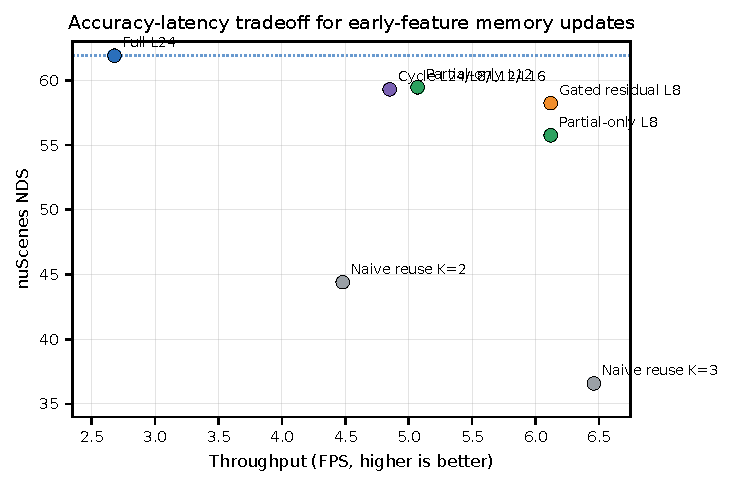
\includegraphics[width=0.82\textwidth]{figures/fig_accuracy_latency_tradeoff.pdf}
    \caption{Accuracy--latency trade-off on DETR3D EVA-02-L. Full L24 encoding maximizes accuracy, while stale reuse is fast but inaccurate. Partial features and temporal updates populate the intermediate operating points; the learned policy attains the strongest measured balance, reaching 60.43 NDS at 5.27 FPS.}
    \label{fig:accuracy-latency}
\end{figure*}

Figure~\ref{fig:accuracy-latency} makes the resulting frontier explicit. Partial depth exposes an accuracy--cost curve: L8 partial-only inference is fastest but loses 6.15 NDS relative to full encoding, whereas moving to L16 recovers 5.06 NDS at lower throughput. The learned policy approaches the L16/full accuracy region while processing many frames more cheaply.

\subsection{Why Temporal Memory Helps}

At L8, adding the gated update raises NDS from 55.75 to 58.23 and mAP from 45.59 to 48.98 without changing the recorded 6.12 FPS. The gain isolates information carried by cached full features. Stale reuse reaches 6.46 FPS but collapses to 36.58 NDS and 21.48 mAP when full encoding occurs every third frame. Current-frame evidence is necessary even when high-level memory exists.

\begin{table}[t]
\centering
\small
\caption{Updater ablation with L8 partial features and the same fixed full-encoding schedule.}
\label{tab:updater-ablation}
\resizebox{\columnwidth}{!}{%
\begin{tabular}{lrrr}
\toprule
Non-full-frame operation & NDS & mAP & FPS \\
\midrule
Partial only & 55.75 & 45.59 & 6.12 \\
Gated residual & \textbf{58.23} & \textbf{48.98} & \textbf{6.12} \\
Cross-attention & 54.33 & 43.58 & 5.95 \\
Gated cross-attention & 57.61 & 48.30 & 5.91 \\
Per-camera attention & 55.04 & 44.30 & 5.99 \\
Inverted attention & 52.91 & 42.49 & 5.90 \\
Gated residual + distillation & 58.08 & 48.69 & 6.12 \\
\bottomrule
\end{tabular}}
\end{table}

The simple gated residual updater outperforms every attention variant. Attention adds 2--4\% latency and does not recover accuracy. Feature distillation changes NDS by $-0.15$ and mAP by $-0.29$ relative to the undistilled gate. These negative results favor a small updater: saved backbone computation should not be replaced by a costly temporal module.


\subsection{Policy Training and Input Ablations}

Unconstrained online-only training is brittle because approximation error can accumulate. Bounding memory age improves the online MLP from 55.21 to 57.94 NDS. Training previous-object features from annotations and replacing them with previous predictions at inference improves the result to 60.05 NDS and 50.61 mAP. Hard-aware class weighting raises accuracy to 60.43 NDS and 51.37 mAP at 5.27 FPS.

Current-frame annotation features do not provide a useful oracle advantage in the evaluated setup: they obtain 57.17 NDS and 47.24 mAP. Previous-frame ground-truth summaries reach 57.38/47.48. The stronger autoregressively-conditioned result appears to come from the training scheme and its interaction with the policy rather than direct access to oracle scene statistics.

\section{Discussion}

An early feature is not merely a cheaper substitute for a final feature. Its best use here is as a current-frame correction to high-level memory. This explains why L8 updating improves substantially over L8 partial-only inference at the same measured throughput.

The policy adds value by selecting where to spend semantic depth. Fixed schedules vary compute with frame index but cannot react to motion or scene change. The improvement over the cyclic schedule suggests that frame-dependent allocation matters beyond average depth. Action-frequency logs are still needed for a strict compute-matched decomposition.

A shallow probe predicts feature similarity accurately, but it is useful only if its cost and subsequent action improve end-to-end detection. Our strongest detector uses previous predictions rather than a current L8 cascade. The probe analysis is therefore evidence for a promising policy input, not an end-to-end speedup claim.

\section{Limitations}

The evaluation uses one detector, one EVA-02-L backbone, one dataset, one image resolution, and one run per setting. Transfer to StreamPETR is supported by the interface design but has not been demonstrated experimentally.

The policy uses full-representation cosine drift as an ordered proxy
for compute demand rather than directly optimizing per-frame
detection regret. Although our analysis shows that high-drift frames
are more sensitive to shallow encoding, small task-critical changes
may still be diluted by global feature aggregation. In addition, the
memory remains defined on the camera image grids and is not explicitly
warped across time. Current partial features, learned gating, and a
maximum memory age limit this error, but large viewpoint or object
motion can still require an early full refresh.

Autoregressive policy conditioning introduces a distribution shift because previous ground-truth summaries are used during training, whereas previous network predictions are used at inference. Absolute ego pose also appears in the current online vector and may encode route-specific correlations.

Throughput values are single-run averages. The profiler synchronizes CUDA around measured regions, but the repository lacks a complete publication protocol with warm-up count, percentile latency, preprocessing boundaries, and confidence intervals. Some probe experiments assume overlap with next-frame processing and are excluded from headline claims. Peak GPU memory, FLOPs, action frequencies, and high-motion failure subsets remain unreported.

\section{Conclusion}

\method{} replaces uniform full-depth image encoding with policy-selected partial computation and dense temporal feature memory. On nuScenes, it reaches 60.43 NDS and 51.37 mAP at 5.27 FPS, retaining most full-encoder accuracy at $1.97\times$ throughput. Controlled ablations show that memory adds value beyond partial features alone and that a simple gated update is more effective than heavier attention variants. Scene-grouped analysis further shows that representation drift is predictable from online signals. Adaptive partial encoding is therefore a practical direction for reducing repeated backbone computation in streaming 3D detection.


\newpage

{\small
\bibliographystyle{plainnat}
\bibliography{main}
}


\newpage

\appendix

\section{Implementation and Training Details}
\label{app:implementation}

\paragraph{Detector interface.}
The controller operates between the image backbone/feature pyramid and the DETR3D sparse head. Full and partial features are lists of tensors with shape $B\times V\times256\times H_s\times W_s$. Scene changes and discontinuities clear the cache. Partial actions project EVA block 8, 12, or 16 through a four-scale pyramid with scale factors $4,2,1,$ and $0.5$.

\paragraph{Updater and policy.}
The updater uses two $1\times1$ convolutions and a residual scale initialized to zero. The MLP uses a 32-dimensional hidden layer and four labels mapped to L8/L12/L16/L24. Base similarity thresholds are 0.90, 0.76, and 0.675 with class weights $1,1,1,3$. The hard-aware model uses thresholds 0.92, 0.80, and 0.72 and weights $1,1.2,2,4$.

\paragraph{Optimization.}
The base detector uses AdamW with learning rate $4\times10^{-4}$, backbone multiplier 0.1, weight decay 0.01, cosine annealing, 500 warm-up iterations, mixed precision, and gradient clipping at norm 35. Training lasts 42,192 iterations with eight GPUs and batch size two per GPU. Temporal runs initialize from the trained DETR3D checkpoint and freeze pretrained detector parameters.

\paragraph{Safety refresh.}
The controller bounds consecutive partial updates by forcing a full encoding after a maximum memory age. This is a safeguard against recurrent error, not the policy contribution.

% \paragraph{Latency protocol.}
% Runs use NVIDIA A100 GPUs with CUDA 11.7, cuDNN 8.5, PyTorch 1.13.1, MMCV 1.7.0, and mixed precision. The profiler synchronizes CUDA around timed regions. no warm-up frames.







\section{Extended Policy Results}
\label{app:policy-results}

\begin{table*}[t]
\centering
\scriptsize
\caption{Completed policy experiments. Accuracy is from validation logs where available; timing is from the experiment ledger. GT inputs denote oracle inference. Autoregressive (Auto-reg) models use previous GT summaries during training and previous predictions at inference. Max age is an implementation safeguard.}
\label{tab:policy-extended}
\resizebox{\textwidth}{!}{%
\begin{tabular}{p{5.1cm}llllrrrr}
\toprule
Policy variant & Inference input & Actions & Max age & Deployable & NDS & mAP & FPS & ms \\
\midrule
Exported 3-level MLP$^{\dagger}$ & online metadata & 8/12/24 & none & yes & 52.60 & 40.27 & 4.15$^{\dagger}$ & 312$^{\dagger}$ \\
Trainable 4-level MLP & online metadata & 8/12/16/24 & none & yes & 55.21 & 44.86 & 4.41 & 226.91 \\
Trainable 4-level MLP & online metadata & 8/12/16/24 & 5 & yes & 57.94 & 48.57 & 4.74 & 212.28 \\
Current-GT oracle & current annotations & 8/12/16/24 & 5 & no & 57.17 & 47.24 & 4.71 & 212.18 \\
Previous-GT oracle, shorter training & previous annotations & 8/12/16/24 & 3 & no & 58.57 & 49.13 & 4.88 & 204.98 \\
Hand-set shallow-drift policy & previous L8 drift & 8/12/16/24 & 4 & yes & 55.65 & 43.86 & 3.49 & 286.66 \\
Trainable MLP + previous L12$^{\ddagger}$ & online + previous L12 & 8/12/16/24 & none & qualified & 55.18 & 44.83 & 4.30 & 232.30 \\
Previous-GT oracle & previous annotations & 8/12/16/24 & 5 & no & 57.38 & 47.48 & 4.60 & 217.22 \\
Auto-reg prediction features & previous predictions & 8/12/16/24 & 5 & yes & 60.05 & 50.61 & 5.17 & 193.35 \\
Auto-reg, hard-aware labels & previous predictions & 8/12/16/24 & 5 & yes & \textbf{60.43} & \textbf{51.37} & \textbf{5.27} & \textbf{189.58} \\
Auto-reg, shorter max age & previous predictions & 8/12/16/24 & 4 & yes & 60.43 & 51.23 & 5.11 & 195.71 \\
\bottomrule
\end{tabular}}

\vspace{0.3em}
\parbox{\textwidth}{\footnotesize $^{\dagger}$The ledger reports 54.30 NDS/47.05 mAP, whereas the available validation log reports 52.60/40.27; its FPS and latency are also mutually inconsistent. The row is excluded from claims. $^{\ddagger}$The ledger excludes the always-computed L12 probe under an overlap assumption, so latency is not directly comparable.}
\end{table*}



\section{Difficulty Classification Analysis}

With fixed cosine thresholds 0.65 and 0.80, an online-metadata MLP obtains 80.4\% accuracy, 63.0\% balanced accuracy, and 59.5\% macro-F1 under scene-grouped cross-validation. Adding current L8 raises these values to 86.5\%, 78.5\%, and 80.0\%. A gradient-boosting oracle with offline metadata and L8 reaches 90.5\%, 86.1\%, and 86.8\%.

On 5,448 frames with previous signals, online metadata plus previous L12 drift obtains 79.9\% macro-F1 with gradient boosting. Adding previous ground-truth summaries raises it to 85.0\%. Threshold sensitivity indicates that $q_{20}/q_{80}$ three-level bins produce 86.7\% macro-F1, while four-level $q_{20}/q_{70}/q_{90}$ bins produce 82.2\%. These diagnostics guide label design but do not replace detector evaluation.

\begin{figure*}[t]
    \centering
    \begin{minipage}[t]{0.49\textwidth}
        \centering
        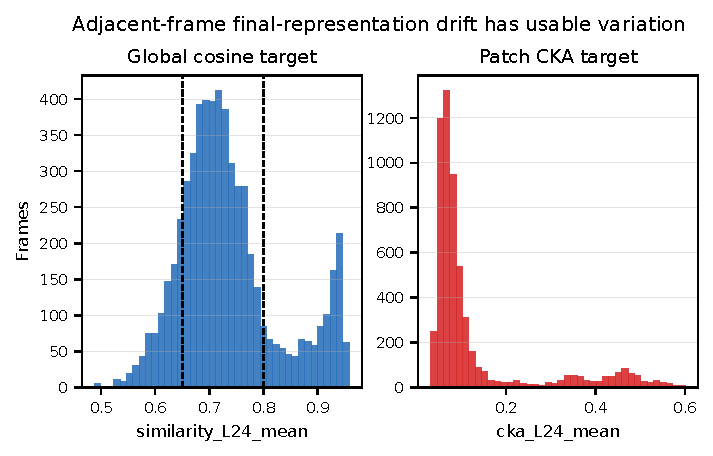
\includegraphics[width=\linewidth]{figures/fig_drift_target_distributions.pdf}
    \end{minipage}\hfill
    \begin{minipage}[t]{0.49\textwidth}
        \centering
        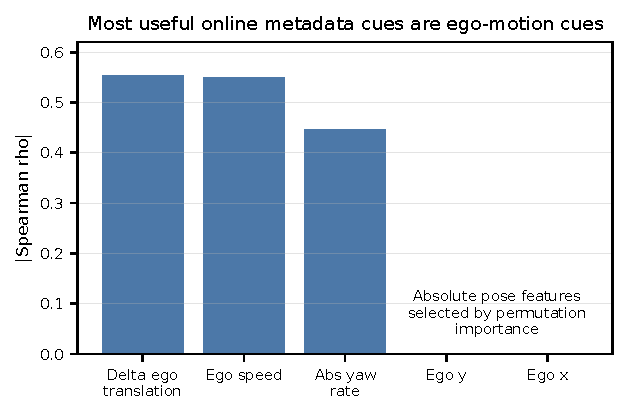
\includegraphics[width=\linewidth]{figures/fig_top_online_metadata_cues.pdf}
    \end{minipage}
    \caption{Policy-signal diagnostics on nuScenes validation frames. \textbf{Left:} adjacent-frame L24 cosine and patch-CKA target distributions; both vary substantially, while measuring different aspects of representation change. \textbf{Right:} strongest online-safe metadata cues for cosine drift. Ego translation, speed, and yaw rate provide physically meaningful evidence before image encoding; feature importance is interpretive rather than causal.}
    \label{fig:policy-diagnostics}
\end{figure*}

\begin{table}[t]
\centering
\small
\caption{Fixed-frequency and partial-depth records.}
\label{tab:fixed-extended}
\resizebox{\columnwidth}{!}{%
\begin{tabular}{lrrrr}
\toprule
Method & NDS & mAP & FPS & ms \\
\midrule
Full encoding every frame & 61.90 & 53.10 & 2.68 & 373.37 \\
Naive reuse, every 2 frames & 44.40 & 31.81 & 4.48 & 206.73 \\
Naive reuse, every 3 frames & 36.58 & 21.48 & 6.46 & 154.82 \\
Partial only, L8 & 55.75 & 45.59 & 6.12 & 161.92 \\
Partial only, L12 & 59.46 & 50.55 & 5.07 & 197.90 \\
Partial only, L16 & 60.81 & 51.96 & 4.24 & 236.08 \\
Fixed gated update, L8 & 58.23 & 48.98 & 6.12 & 163.50 \\
Variable-depth cycle & 59.30 & 50.05 & 4.85 & 206.29 \\
\bottomrule
\end{tabular}}
\end{table}



\section{Qualitative Evaluation}

\begin{figure*}[t]
    \centering
    \fcolorbox{red}{white}{\parbox{0.94\textwidth}{\centering\color{red}
    \textbf{Manual qualitative figure placeholder.} Select three nuScenes sequences: stable cruising, a sharp ego turn, and dense traffic with new objects. Show four timestamps with camera predictions, bird's-eye-view boxes, selected action, policy confidence, and memory age. Add one failure case where the policy exits too early and misses a newly visible nearby object.}}
    \caption{Requested qualitative comparison of policy decisions and 3D predictions across temporal regimes.}
    \label{fig:qualitative}
\end{figure*}

\subsection{Which Signals Predict Required Depth?}

We analyze 5,869 adjacent frame pairs from 150 nuScenes validation scenes. Five-fold cross-validation groups frames by scene. The cosine target is mean adjacent L24 similarity; the CKA target uses patch features only. We compare online metadata, annotation-derived offline metadata, and a current-frame L8 similarity probe.

\subsection{Does Representation Drift Indicate Compute Demand?}
\label{sec:drift-demand}

The policy is supervised by representation drift rather than directly
by detection loss. We therefore first test whether this target
identifies frames on which shallow computation is insufficient. For
each candidate depth $\ell\in\{8,12,16\}$, we evaluate the detector
under the same refresh interval and preceding memory state and measure
its degradation relative to full-depth inference:
\begin{equation}
\Delta_t^\ell
=
\mathcal{E}(\widehat{Y}_t^\ell,Y_t)
-
\mathcal{E}(\widehat{Y}_t^{24},Y_t),
\end{equation}
where $\mathcal{E}$ is \rednote{state the per-frame detection loss or
prediction-discrepancy measure used in the analysis}.

Figure~\ref{fig:drift-vs-degradation} groups frames into quantiles of
the full-representation drift $d_t^L$. Shallow L8 inference changes
only modestly in the lowest-drift intervals but degrades increasingly
as drift grows. L12 and L16 exhibit the same trend with progressively
smaller degradation. The Spearman correlations between $d_t^L$ and
$\Delta_t^\ell$ are \rednote{L8 correlation},
\rednote{L12 correlation}, and \rednote{L16 correlation},
respectively. These results do not establish that cosine drift is a
perfect task-aware oracle; rather, they show that it is an informative
ordered proxy for the amount of semantic recomputation required.

\begin{figure*}[t]
    \centering
    \includegraphics[width=0.8\linewidth]
    {figures/scene01_frame03_pred.png}
    \caption{
    prediction using policy \mk{need to compare to GT}}
    \label{fig:example}
\end{figure*}


\begin{figure*}[t]
    \centering
    \includegraphics[width=0.8\linewidth]
    {figures/scene01_frame03_feature_L8.png}
    \caption{\mk{placeholder}
    Relating representation drift to insufficient encoder depth.
    Frames are grouped by full L24 drift. The curves show detection
    degradation for L8, L12, and L16 relative to L24 under the same
    memory-refresh protocol. High-drift frames are more sensitive to
    shallow encoding, while deeper partial representations reduce the
    degradation.
    }
    \label{fig:drift-vs-degradation}
\end{figure*}

\subsection{Can Drift Be Predicted Before Encoding?}

We next evaluate which signals predict the current full-representation
drift $d_t^L$. We group cross-validation folds by scene and distinguish
three information regimes:
\begin{itemize}[leftmargin=*]
    \item \textbf{Online metadata:} relative ego motion, scene age,
    memory age, and previous action.
    \item \textbf{Lagged online state:} previous detections and L8
    drift measured between $t-2$ and $t-1$. These are available before
    encoding frame $t$.
    \item \textbf{Current-frame or offline cues:} current L8 features
    and annotation-derived statistics, used only as diagnostic upper
    bounds.
\end{itemize}

The main deployable comparison should report online metadata alone,
online metadata with previous detections, and the full policy input
including lagged L8 drift. Current-frame L8 similarity is reported
separately as a cascade upper bound rather than as an input to the
headline policy.

Replace the current policy table with a structure like:

\begin{table*}[t]
\centering
\small
\caption{\mk{need to review and add real numbers, this is approximationv}Policy and control ablations. All learned policies use the
same memory updater. Lagged L8 uses cached features from frames
$t-2$ and $t-1$ and therefore requires no current-frame probe.
Average depth and full-action frequency expose differences in compute
allocation beyond measured latency.}
\label{tab:policy-ablation}
\begin{tabular}{lccccccccc}
\toprule
Policy variant &
Prev. det. &
Lagged L8 &
Scene age &
Max age &
Avg. depth &
L24 (\%) &
NDS &
mAP &
ms \\
\midrule
Cyclic schedule            & -- & -- & -- & \rednote{} & \rednote{} & \rednote{} & 59.30 & 50.05 & 206.3 \\
Random, matched actions     & -- & -- & -- & \rednote{} & \rednote{} & \rednote{} & \rednote{} & \rednote{} & \rednote{} \\
Metadata only               &    &    & \checkmark & $\infty$ & \rednote{} & \rednote{} & 55.21 & 44.86 & 226.9 \\
Metadata + bounded age      &    &    & \checkmark & 5 & \rednote{} & \rednote{} & 57.94 & 48.57 & 212.3 \\
+ previous detections       & \checkmark &    & \checkmark & 5 & \rednote{} & \rednote{} & 60.05 & 50.61 & 193.4 \\
+ lagged L8 drift           & \checkmark & \checkmark & \checkmark & 5 & \rednote{} & \rednote{} & \rednote{} & \rednote{} & \rednote{} \\
+ hard-aware supervision    & \checkmark & \checkmark & \checkmark & 5 & \rednote{} & \rednote{} & 60.43 & 51.37 & 189.6 \\
\method{} accuracy setting  & \checkmark & \checkmark & \checkmark & \rednote{} & \rednote{} & \rednote{} & 60.43 & 54.41 & 195.7 \\
\bottomrule
\end{tabular}
\end{table*}


\begin{table}[t]
\centering
\small
\caption{Grouped-CV regression of final-feature similarity. Values are mean $\pm$ standard deviation across five scene folds. Offline metadata is an oracle. MAE is target-specific.}
\label{tab:signal-regression}
\resizebox{\columnwidth}{!}{%
\begin{tabular}{llrr}
\toprule
Target & Policy features & $R^2$ & MAE \\
\midrule
\multirow{4}{*}{Cosine}
 & Online metadata & $0.706\pm0.043$ & $0.0391\pm0.0020$ \\
 & Online + current L8 & $0.902\pm0.021$ & $0.0216\pm0.0010$ \\
 & Offline metadata & $0.853\pm0.037$ & $0.0268\pm0.0014$ \\
 & Offline + current L8 & $0.952\pm0.010$ & $0.0149\pm0.0006$ \\
% \midrule
% \multirow{4}{*}{Patch CKA}
%  & Online metadata & $0.889\pm0.037$ & $0.0231\pm0.0008$ \\
%  & Online + current L8 & $0.933\pm0.017$ & $0.0197\pm0.0015$ \\
%  & Offline metadata & $0.875\pm0.062$ & $0.0221\pm0.0016$ \\
%  & Offline + current L8 & $0.943\pm0.023$ & $0.0173\pm0.0018$ \\
\bottomrule
\end{tabular}}
\end{table}

Online metadata explains 70.6\% of cosine-similarity variance. Adding L8 reduces MAE by 44.8\% and raises $R^2$ to 0.902. For CKA, the online baseline reaches $R^2=0.889$, and L8 raises it to 0.933. The result supports a cascade in which metadata makes a pre-encoding decision and L8 resolves ambiguous cases, provided that probe cost is measured.


As visualized in \cref{fig:policy-signals}, the L8 representation is not only a cheaper detector feature: it is also evidence about whether further semantic processing is required. Ego translation and speed dominate permutation importance for metadata-only cosine prediction. For CKA, absolute yaw rate has Spearman correlation $-0.651$, and L8 similarity correlates with final CKA at $0.673$. Cosine and CKA have Spearman correlation $0.501$, so they measure related but distinct changes. Additional target and cue visualizations appear in \cref{fig:policy-diagnostics}.


\begin{figure*}[t]
    \centering
    \begin{minipage}[t]{0.49\textwidth}
        \centering
        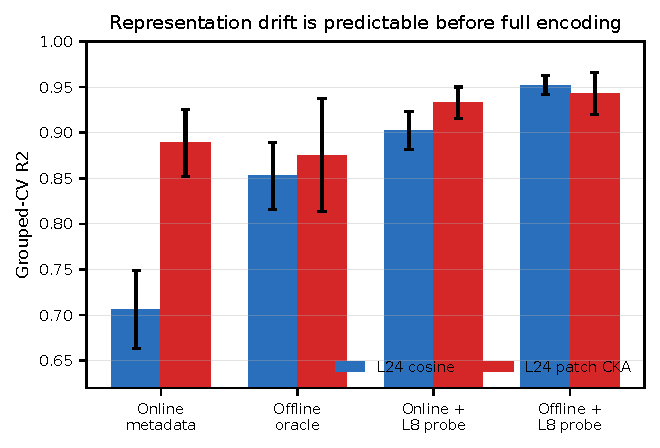
\includegraphics[width=\linewidth]{figures/fig_drift_predictability_r2.pdf}
    \end{minipage}\hfill
    \begin{minipage}[t]{0.49\textwidth}
        \centering
        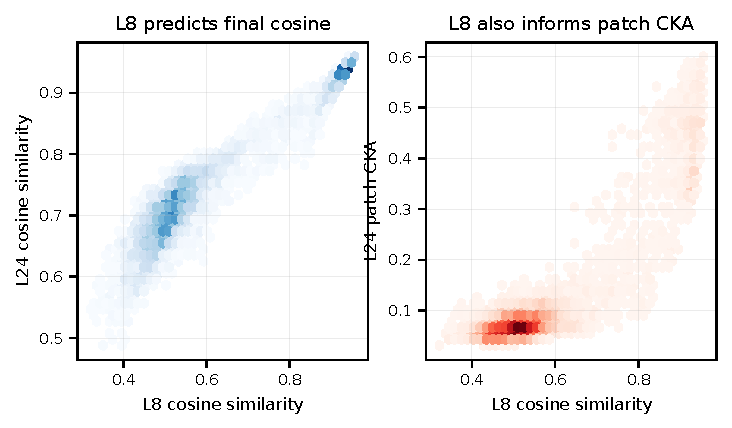
\includegraphics[width=\linewidth]{figures/fig_l8_probe_vs_final_drift.pdf}
    \end{minipage}
    \caption{Evidence for policy inputs. \textbf{Left:} scene-grouped cross-validation for predicting final L24 representation drift. Online metadata is predictive, and adding a current L8 probe improves both cosine and patch-CKA targets. \textbf{Right:} current L8 similarity versus final L24 drift. The early representation is informative before committing to deeper encoding, which gives partial encoding a second role as a cascade measurement.}
    \label{fig:policy-signals}
\end{figure*}

\end{document}
